\graphicspath{{1egypt/pics/}}

\section{Ancient Egypt}

\boldinline{Summary}

\begin{itemize}\itemsep0pt
  \item Recorded civilization in Nile valley from c.\,3150\BC.
  \item Conquered 322\BC{} by Alexander the Great (Greece/Macedonia).
  \item Became a Roman province in 30\BC{} under Cleopatra. 
  \item Discovery of the Rosetta Stone (\AD 1799) containing Greek, hieroglyphic and demotic (post hieratic, cursive) Egyptian script, allowed translation of ancient Egyptian writing.
  \item Primary mathematical sources: Rhind/Ahmes (A'h-mose) papyrus c.\,1650\BC{} and the Moscow papyrus c.\,1700\BC.\footnote{Rhind was a Scottish egyptologist. Ahmes was the name of the scribe who wrote/copied the papyrus. The Moscow papyrus is named because it was sold to the Moscow Museum of Fine Art; its author is unknown.} Part of the Rhind papyrus is shown below. It contained two tables: unit fraction representations of all $\frac 2n$ for $n<100$ (ish) and expressions for $\frac 3{10},\frac 4{10},\ldots,\frac 9{10}$ in terms of unit fractions. Also included were around 100 worked problems. Scribes would learn the method by copying previous problems and changing the numbers.\par
  The Moscow papyrus is shorter and more focused on geometric problems.
  \begin{center}
  	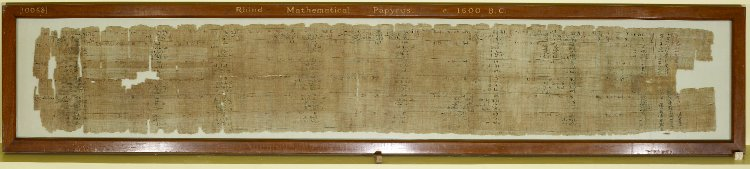
\includegraphics[scale=0.4]{rhindwhole.jpg}\\
  	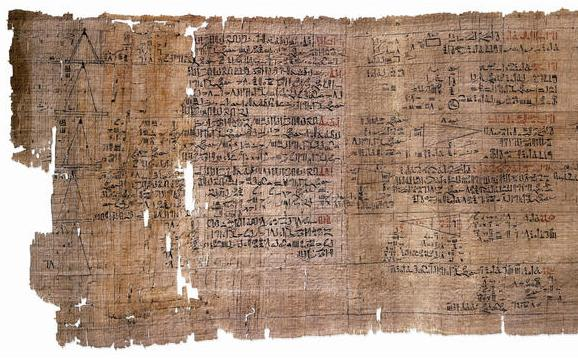
\includegraphics[scale=0.8]{Rhind_Mathematical_Papyrus.jpg}
  \end{center}
  \item Few other primary sources. Egyptians wrote on papyrus (plant-based form of paper) which decomposes. Other Egyptian mathematics was likely absorbed uncredited by the Greeks.
  \item Practical/non-theoretical: worked problems on sums, linear equations, construction and land-measurement (tax-collection). No clear distinction between exact and approximate solutions.
\end{itemize}

\goodbreak


\boldsubsection{Notation \& Egyptian Fractions}

The ancient Egyptians had two distinct systems for enumeration: \emph{hieroglyphic} (dating at least to 5000\BC) and \emph{hieratic} (c.\,2000\BC). These changed over time, so we give only one version.

\begin{minipage}[t]{0.64\linewidth}\vspace{0pt}
	\boldinline{Hierogylphic enumeration} Essentially decimal symbols for numerals/powers of 10.
	\begin{itemize}\itemsep0pt
	  \item Could be written in any direction: top-to-bottom, right-to-left, etc., or just lumped together: e.g.\vspace{-3pt}
		\[
			2349=\egyptify{0}{0}{0}{2}{3}{4}{9}
		\]\vspace{-23pt}
	  \item Slow to write, numbers take up a lot of space.
	\end{itemize}
\end{minipage}
\hfill
\begin{minipage}[t]{0.35\linewidth}\vspace{0pt}
	\flushright
	\begin{tabular}{c|c}
		Numeral&Hieroglyph\\\hline
		1&$\egone{1}$\\
		10&$\egten{1}$ (heel bone)\\
		100&$\eghun{1}$ (snare)\\
		1000&$\egtho{1}$ (lotus flower)\\
		10000&$\egtentho{1}$ (finger)\\
		100000&$\eghuntho{1}$ (fish)\\
		1000000&$\egmil{1}$ (person)
	\end{tabular}
\end{minipage}
\bigbreak


\begin{minipage}[t]{0.5\linewidth}\vspace{0pt}
	\boldinline{Hieratic enumeration}
	
	We will largely ignore this since it is written cursively.
	\begin{itemize}\itemsep0pt
	  \item Different symbols for 1--9, 10--90, 100--900 etc., mapped onto hieratic alphabet.
	  \item System copied later by the Greeks with their own alphabet.
	  \item Pros: less space, easier to write with ink, each number requires fewer symbols.
		\item Cons: More symbols, slower calculations.
	\end{itemize}
\end{minipage}
\hfill
\begin{minipage}[t]{0.49\linewidth}\vspace{0pt}
	\flushright
	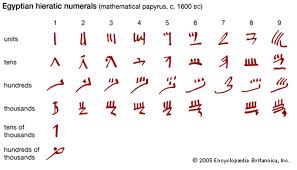
\includegraphics[scale=0.75]{hieratic.jpg}
\end{minipage}
\medbreak

For instance, $23$ would be written (approximately!) $|||\cl{\wedge}$.\smallbreak

The Eygptians had no numeral for zero, though the hieroglyph \emph{nfr} (beautiful/perfect) was used to denote, for instance, the base floor of a building or to indicate balanced books in accounting.
\vspace{-5pt}


\boldinline{Fractions}

Ancient Egyptians worked almost entirely with \emph{reciprocals} of integers ($\frac 1n$ where $n\in\N$). In modern times, any fraction represented as a sum of reciprocals is called an \emph{Egyptian fraction}; their theory is still actively researched. For instance
\[
	\frac 12+\frac 14+\frac 15
\]
is a representation of $\frac{19}{20}$ as an Egyptian fraction.\smallbreak
In hieratic notation, a dot was placed above to denote the reciprocal: e.g., $\dot{\wedge}$ is $\frac 1{10}$.\par

\begin{minipage}[t]{0.53\linewidth}\vspace{0pt}
	In hieroglyphs, a reciprocal was represented by placing an oval over a numeral. We do this with a bar: e.g. $\cl 2=\frac 12$. As with integers, combinations of fractions could be written in any order/direction.
	\smallbreak
	The only non-reciprocal fractions with special symbols were $\frac 23$ and $\frac 34$, and these only appeared late in Egyptian civilization.\footnotemark{} %If necessary, we can write $\cl{\cl 3}=\frac 23$ in modern notation. 
\end{minipage}
\hfill
\begin{minipage}[t]{0.46\linewidth}\vspace{0pt}
	\flushright\def\arraystretch{0.9}
	\begin{tabular}{c|c|c@{}}
		Fraction&Hieroglyph&Modern\,\,\\\hline
		\raisebox{3pt}{$\frac 13$}&\egfrac{\egone{3}}&$\cl 3$\\
		\raisebox{3pt}{$\frac 1{41}$}&\egfrac{\egyptify{0}{0}{0}{0}{0}{4}{1}}&$\cl{41}$\\
		\raisebox{3pt}{$\frac 1{103204}$}&\egfrac{\egyptify{0}{1}{0}{3}{2}{0}{4}}&$\cl{103204}$\\
		\raisebox{3pt}{$31+\frac 12+\frac 1{25}$}&\egfrac{\egone{5}\egten{2}} \ \egfrac{\egone{2}}\ \ \egone{1}\egten{3}
		&$\cl{25}\ \ \cl 2\ \ 31$
	\end{tabular}
\end{minipage}
\bigbreak

\footnotetext{For instance an oval over one-and-a-half sticks for $\frac 23$, and an oval over three short-long-short sticks for $\frac 34$.}

\goodbreak


\begin{minipage}[t]{0.7\linewidth}\vspace{0pt}
	The Rhind papyrus contains a table, of which we reproduce part, showing how to express $\frac 2n$ as Egyptian fractions for all odd integers $n<100$. The first column denotes $n$, and the remaining columns the Egyptian fraction representation. For instance, the first row states
	\[
		\frac 25=\frac 13+\frac 1{15}\hfill(\text{\egfrac{\egone{3}} \egfrac{\egone{5}\egten{1}}}\qquad\cl 3\ \cl{15})
	\] 
\end{minipage}
\hfill
\begin{minipage}[t]{0.29\linewidth}\vspace{0pt}
	\flushright
	$\begin{array}{c|cccccc}
		%\frac 2n&\frac 1p&+&\frac 1q&+&\frac 1r&+\cdots\\\hline
		5&3&&15&&&\\
		7&4&&28&&&\\
		9&6&&18&&&\\
		11&6&&66&&&\\
		13&8&&52&&104&\\
		15&10&&30&&&%\\
		%\vdots&&&&&&
	\end{array}$
\end{minipage}
\bigbreak

There are several approaches to finding Egyptian fraction representations, and it can be proved that any fraction may be written in such a form. If the denominator is odd, then a simple place to start is with
\[
	\frac 2{mn}=\frac 1{mr}+\frac 1{nr}\quad\text{where}\quad r=\frac{m+n}2
\]
Most lines in the Rhind table follow this formula, but not all. Note also that the formula often permits multiple representations.
\begin{itemize}
  \item The line for $\frac 25$ has $m=1$, $n=5$ and $r=3$; this is unique up to reordering.
  \item $\frac 29$ may be represented
  \[
  	\frac 29=
  	\begin{cases}
  		\frac 19+\frac 19&(m,n,r)=(3,3,3)\\
  		\frac 15+\frac 1{45}&(m,n,r)=(1,9,5) 	
  	\end{cases}
  \]
  The first of these is essentially useless and the second is not the expression from the table.
  \item In the table, $\frac 2{13}$ is written as a sum of three reciprocals instead of two.
\end{itemize}

The table reduced the need to divide and sped up the computation of harder fractions: for instance,
\[
	\frac 5{13} =2\cdot\frac 2{13}+\frac 1{13} =2\left(\frac 18+\frac 1{52}+\frac 1{104}\right)+\frac 1{13} =\frac 14+\frac 1{13}+\frac 1{26}+\frac 1{52}
\]



 
\boldsubsection{Egyptian Calculations \& Example Problems}

\boldinline{Addition/Subtraction} With hieroglyphs this is simple: Write out numbers one above another and count up the symbols! Replace 10 of one by the next symbol. For subtraction, one might need to convert a larger symbol to 10 of a smaller one. Essentially this is `carrying.' A special symbol was used to denote both addition and subtraction: its meaning changed depending on the direction the text was read.

\boldinline{Multiplication} This relied on a base-two algorithm. To compute $ab$:
\begin{enumerate}
  \item Write $1,b$
  \item Repeatedly double each until the first term is about to exceed $a$
  \item Determine powers of 2 that sum to $a$
  \item Sum the corresponding multiples of $b$
\end{enumerate}

\goodbreak

For example, to compute $13\cdot 15$, we construct a table where the checked rows are summed.
\[
	\begin{array}{r@{\qquad}r@{\qquad}c}
		1&15&\checkmark\\
		2&30&\\
		4&60&\checkmark\\
		8&120&\checkmark
	\end{array}
	\quad\implies 13\cdot 15=(1+4+8)\cdot 15=15+60+120=195
\]
Note how $13=1+4+8=2^0+2^2+2^3$ is essentially the binary representation. We stopped at the fourth row since another doubling would have resulted in the first term (16) exceeding 13. We could instead have reversed the roles of the factors:
\[
	\begin{array}{r@{\qquad}r@{\qquad}c}
		1&13&\checkmark\\
		2&26&\checkmark\\
		4&52&\checkmark\\
		8&104&\checkmark
	\end{array}
	\quad\implies 15\cdot 13=(1+2+4+8)\cdot 13=13+26+52+104=195
\]
All you need is addition and the ability to multiply by 2!


\boldinline{Division} This also relies on doubling/halving, though the answer is non-unique and might require some creativity. To find $\frac ab$, think about solving the problem $a=bx$ and apply a variant of the multiplication algorithm to find multiples of $b$ summing to $a$. Here are some examples.

\begin{enumerate}
	\item To compute $260\div 13$, we repeatedly double 13 until terms in the right column sum to 260.
	\[
		\begin{array}{r@{\qquad}r@{\qquad}c}
			1&13\\
			2&26\\
			4&52&\checkmark\\
			8&104\\
			16&208&\checkmark
		\end{array}
	\]
	Since $260=208+52$ we conclude that $260\div 13=16+4=20$

	%\item $\frac{271}{13}$: We would continue the above table, noting that

	\item To find $5\div 13$ we start by dividing by 2 with the intent of making terms in the right column sum to 5.
	\[
		\begin{array}{r@{\qquad}r@{\qquad}c}
1&13\\
			\cl 2&6\ \cl 2\\
			\cl 4&3\ \cl 4&\checkmark\\
			\cl 8&1\ \cl 2\ \cl 8&\checkmark
		\end{array}
	\]
	Since $(3\ \cl 4)+(1\ \cl 2\ \cl 8)=4\ \cl 2\ \cl 4\ \cl 8$ is $\cl 8$ ($\frac 18$) short of what we want, we continue the table in a different way. First divide by 13, then continue halving until we obtain the desired $\cl 8$ in the right column.
	\[
		\begin{array}{r@{\qquad}r@{\qquad}c}
			\cl{13}&1\\
			\cl{26}&\cl 2\\
			\cl{52}&\cl 4\\
			\cl{104}&\cl 8&\checkmark
		\end{array}
	\]
	We conclude that $5\div 13=\cl 4\ \cl 8\ \cl{104} =\frac 14+\frac 18+\frac 1{104}$. We could have proceeded differently to obtain the same result as followed from the Rhind table:
	\[
		5=(3\ \cl 4)+1+\cl 2+\cl 4\implies 5\div 13=\cl 4\ \cl{13}\ \cl{26}\ \cl{52}
	\]
\end{enumerate}

\goodbreak



\boldinline{Practical application: Loaf-splitting}

A typical Egyptian problem might involve determining how to split 5 loaves among 13 people. The previous calculation tells us that we could give each person $\frac 14+\frac 18+\frac 1{104}$ of a loaf. This might seem complicated but it has some advantages over the modern approach where we'd first cut each loaf into 13 equal pieces:
\begin{itemize}
  \item The large chunks of bread are created by repeatedly cutting in half: this is easy to do accurately, whereas cutting 13\th{} parts is difficult! The remaining 104\th{} parts of a loaf would probably be ignored as crumbs.
  \item The Egyptian approach only requires 34 cuts, as opposed to 60 in the modern style.
\end{itemize}



\boldinline{Linear equations}

Another common type of problem was how to solve linear equations. Solutions were based on the method of \emph{false position.} Essentially one guesses an approximate solution, then modifies it until it works. Here is problem 24 of the Rhind papyrus.
\begin{quote}
	A heap plus a seventh of a heap is nineteen. What is the heap?
\end{quote}
In modern algebra, representing `heap' by $x$, we wish to solve $x+\frac 17x=19$. Here is the Egyptian method.\par

\begin{minipage}[t]{0.69\linewidth}\vspace{0pt}
	\begin{enumerate}
  	\item Guess intelligently: $x=14$ is easy to divide by 7 and we obtain $x+\frac 17 x=16$
  	\item Correct our guess: We want 19, not 16, so we multiply our guess (14) by $\frac{19}{16}=1\ \cl 8\ \cl{16}$ to obtain the correct answer
  	\[
  		x=2\ \cl 4\ \cl 8 +4\ \cl 2\ \cl 4+ 9\ \cl 2 =16\ \cl 2\ \cl 8
  	\]
	\end{enumerate}
\end{minipage}
\hfill
\begin{minipage}[t]{0.3\linewidth}\vspace{0pt}
	\hfill 
	\[
		\begin{array}{r@{\qquad}r@{\qquad}c}
			1&1\ \cl 8\ \cl{16}\\
			2&2\ \cl 4\ \cl 8&\checkmark\\
			4&4\ \cl 2\ \cl 4&\checkmark\\
			8&9\ \cl 2&\checkmark
		\end{array}
	\]
\end{minipage}\medbreak

Compare this with the `modern' method:
\[
	x+\frac 17x=19\implies \frac 87x=19\implies x=\frac{7\cdot 19}8 =\frac{133}8 =\frac{128+5}8= 16\frac 58
\]
Are the any benefits to the Egyptian approach?

\begin{minipage}[t]{0.67\linewidth}\vspace{0pt}
	\boldinline{Geometry}
	
	Problem 48 in the Rhind papyrus involves using an octagon to approximated the area of a circle. A square of side 9 is drawn, where each side is split into thirds and the four corner squares are cut in half. The area of the octagon is then \[81-18=63\]
	Since the area of the circle is $\frac{81\pi}4$, this amounts to the approximation $\pi\approx\frac{28}9=3.11111\ldots$\smallbreak
	
	Problem 50 compares the same circle to a square of side 8: essentially $\frac{81\pi}4\approx 64$ which corresponds to $\pi\approx \frac{256}{81}=3.16049\ldots$
\end{minipage}
\hfill
\begin{minipage}[t]{0.32\linewidth}\vspace{0pt}
	\flushright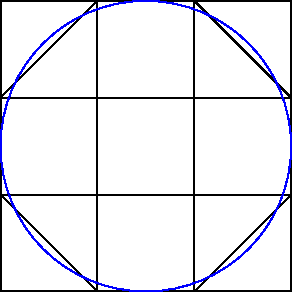
\includegraphics{egypt-octagon}
\end{minipage}\medbreak


No explanation is given as to what inspired these methods, nor whether the scribes understood that these were only approximations.

\goodbreak

\begin{minipage}[t]{0.69\linewidth}\vspace{0pt}
	Other problems computed/approximated areas and volumes of triangles, quadrilaterals, boxes, cylinders, and truncated pyramids. Again, these were worked examples without general formulæ. The Egyptians even had a notion of cotangent which they called the \emph{seked,} useful for describing and calculating slopes.
\end{minipage}
\hfill
\begin{minipage}[t]{0.3\linewidth}\vspace{0pt}
	\flushright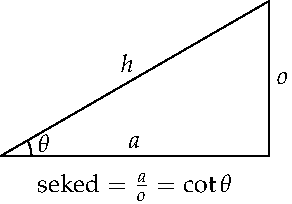
\includegraphics[scale=0.95]{geo-01-seked}
\end{minipage}


\goodbreak


\begin{exercises*}{}{}
	Most of these problems are taken from the `official' textbook.
	\begin{enumerate}
	  \item %[1-2]
	  Use Egyptian techniques to multiply 34 by 18 and to divide 93 by 5.
	  
	  \item %[1-4]
	  Use Egyptian techniques to multiply $\cl{28}$ by $1+\cl 2+\cl 4$ (problem 9 of the Rhind papyrus).
	  
	  \item %[1-8]
	  A part of the Rhind papyrus table for division by 2 reads as follows:
	  \[
	  	2\div 11=\cl6+\cl{66},\qquad 2\div 13=\cl 8+\cl{52}+\cl{104},\qquad 2\div 23=\cl{12}+\cl{276}
	  \]
	  The calculation of $2\div 13$ is given below, where the right hand side is a modern rendering, and the terminal `2' indicates that the last entry in the right-hand column is indeed 2:
	  \begin{quote}
	  	\def\arraystretch{0.8}
		  \begin{tabular}{@{}l@{\qquad\quad}l@{\qquad\qquad\qquad}l@{\qquad}l}
			  \egone{1}
			  	&\egone{3}\egten{1}
			  	&1
			  	&13\\
				\egfrac{\egone{2}}
					&\egone{6}\ \egfrac{\egone{2}}
					&$\cl 2$
					&$6\ \cl{2}$\\
				\egfrac{\egone{4}}
					&\egone{3}\ \egfrac{\egone{4}}
					&$\cl 4$
					&$3\ \cl 4$\\
			  \egfrac{\egone{8}}
			  	&\egone{1}\  \egfrac{\egone{2}}\ \egfrac{\egone{8}}
			  	&$\cl 8$
			  	&$1\ \cl 2\ \cl 8$\\
			  \egfrac{\egone{2}\egten{5}}
			  	&\egfrac{\egone{4}}
			  	&$\cl{52}$&$\cl 4$\\
			  \egfrac{\egone{4}\eghun{1}}
			  	&\egfrac{\egone{8}}
			  	&$\cl{104}$&$\cl 8$\\
			 	\egfrac{\egone{8}}\ \egfrac{\egone{2}\egten{5}}\ \egfrac{\egone{4}\eghun{1}}
			 		&\egone{1}\ \egfrac{\egone{2}}\ \egfrac{\egone{4}}\,\egfrac{\egone{8}}\ \egfrac{\egone{8}}
			 		&$\cl 8\ \cl{52}\ \cl{104}$
			 		&$1\ \cl 2\ \cl 4\ \cl 8\ \cl 8$\\
			  &\egone{2} 
			  	& 
			  	&2
	  	\end{tabular}
	  \end{quote}
	  
	  Perform similar calculations for $2\div 11$ and $2\div 23$.\par
	  (\emph{If you want the exact results from the papyrus, you'll need to work with $\frac 23$: denote this by $\cl{\cl 3}$})
	  
	  \item Draw a picture of 5 loaves to help describe how the Egyptians might have divided them between seven people.
	  
	  \item%[1-10]
	  Use the method of false position to solve problem 28 of the Rhind papyrus:
	  \begin{quote}
	  	A quantity and its $2/3$ are added together, and from the sum $1/3$ of the sum is subtracted, and 10 remains. What is the quantity?
	  \end{quote}

	  \item %[1-12]
	  Calculate a quantity such that if it is taken two times along with the quantity itself, the sum comes to 9  (problem 25 of the Moscow papyrus).

		\item\begin{enumerate}
		  \item Find all ways in which $\frac 2{13}=\frac 1a+\frac 1b$ can be written as a sum of reciprocals ($a\le b\in\N$).
		  \item Repeat your calculation for $\frac 2p$ whenever $p$ is an odd prime.
		\end{enumerate}
	\end{enumerate}
\end{exercises*}

